\begin{figure}
	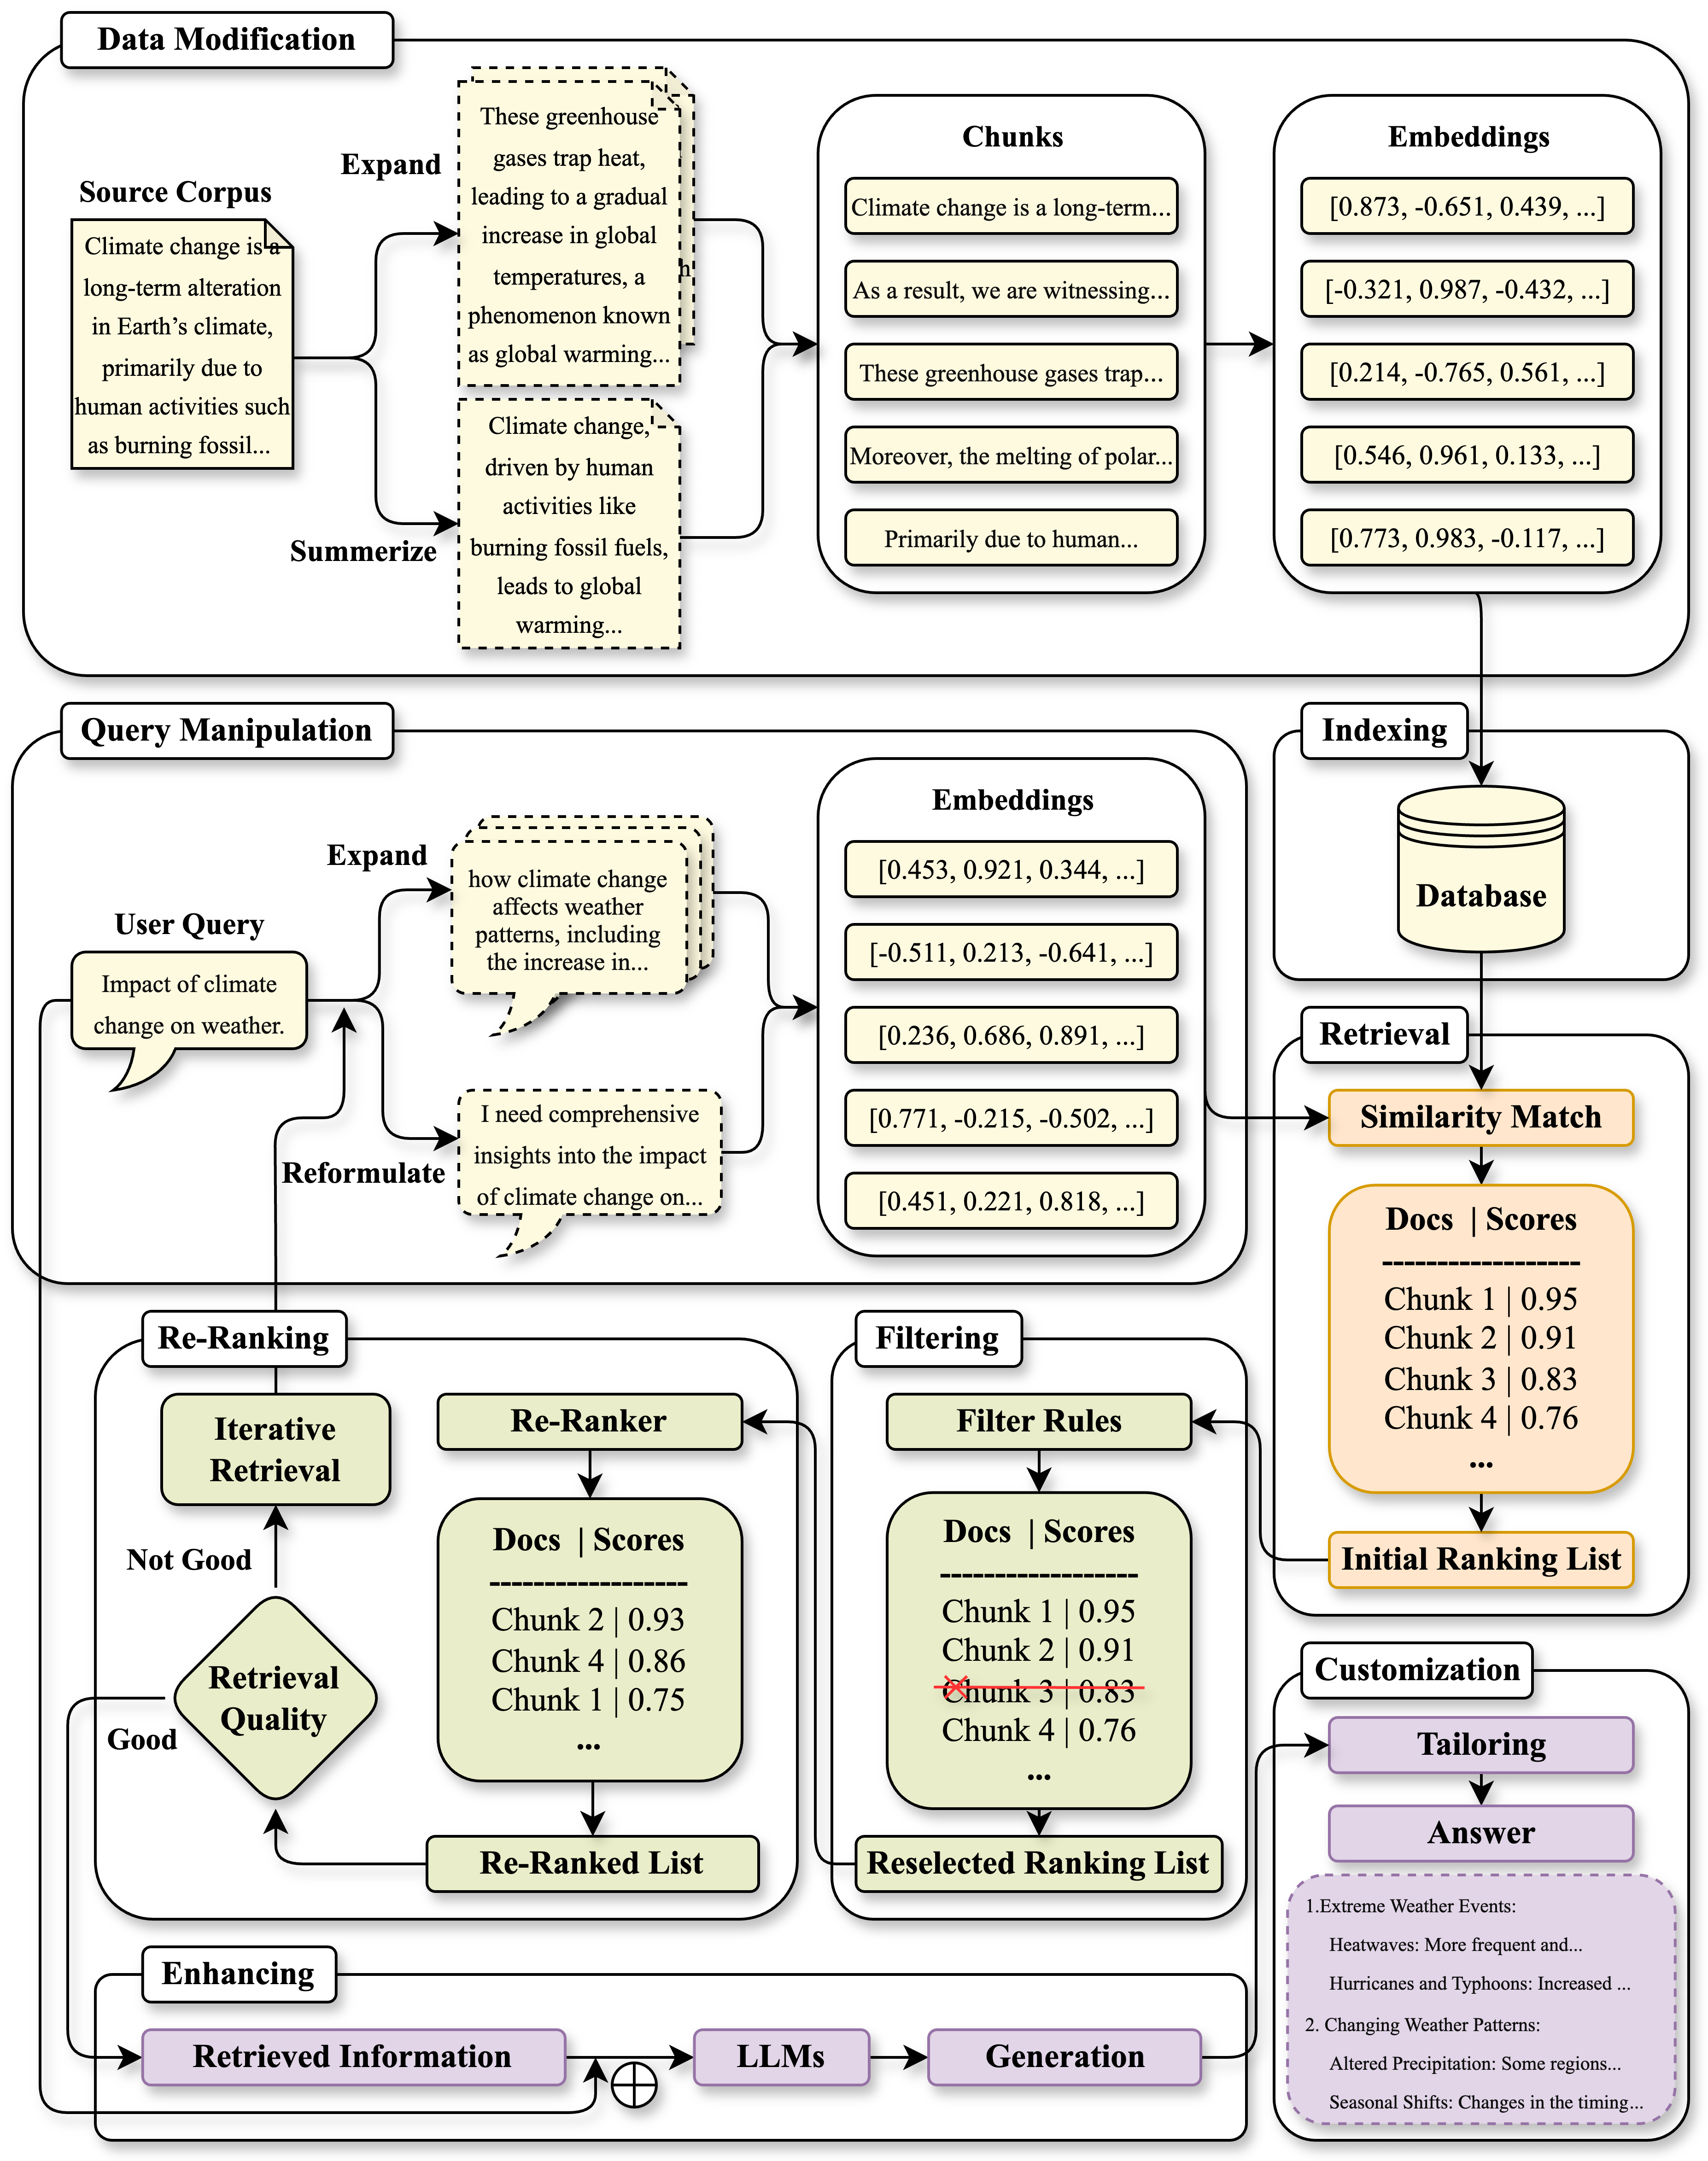
\includegraphics[width=0.85\textwidth]{Figures/RAG_framework.png}
	\caption{An example of a typical RAG framework with interative retrieval strategy.}
	\label{fig:rag_framework}
\end{figure}

\subsection{Search \& Ranking}
The search and ranking process within RAG is crucial for improving the relevance and accuracy of generated outputs. Several methodologies have been developed to refine this process, each contributing unique strategies for enhancing retrieval and ranking. For example, Atlas \cite{izacard2023atlas} and AAR \cite{yu2023augmentationadapted} both aim to improve the relevance of retrieved documents, but they approach this challenge differently. Atlas focuses on optimizing the retriever's ability to select contextually relevant documents, especially in new domains with limited data, by employing few-shot learning techniques such as Attention Distillation and Perplexity Distillation. AAR, on the other hand, adapts retrieval preferences to better align with the requirements of LLMs, enhancing retrieval generalization across tasks by training a smaller source model.

Additionally, IRCOT \cite{trivedi2023interleaving} and FLARE \cite{jiang2023active} introduce dynamic interactions within the retrieval process, albeit with distinct goals. IRCOT integrates retrieval with chain-of-thought (CoT) reasoning, interleaving these processes to ensure that each retrieval step supports the ongoing reasoning task. FLARE, in contrast, adopts a confidence-based active retrieval mechanism, dynamically triggering retrieval when the model generates low-confidence tokens. This approach is particularly useful in scenarios where model confidence varies, as it allows the system to fetch additional information to resolve uncertainties during the generation process.

When addressing domain-specific retrieval challenges, SURGE \cite{kang2023knowledge} and PRCA \cite{yang2023prca} offer different solutions. SURGE uses a subgraph retriever to extract relevant subgraphs from knowledge graphs, integrating structured data into the retrieval process to improve the contextual understanding of generated responses. The relational structure of knowledge graphs allows for more accurate and informed retrieval. PRCA, in contrast, focuses on domain-specific abstractive summarization, using a reward-driven approach to refine the retrieved content. This strategy is designed to optimize content for the generator, particularly in scenarios where the generator functions as a black box, thereby enhancing alignment between retrieval and generation.

MEMWALKER \cite{chen2023walking} presents a unique approach to handling long-context question answering by incorporating an internal search and ranking mechanism within a memory tree structure. This method navigates extensive memory stores, ensuring that the most relevant information is retrieved and used for complex queries. Unlike other methods, MEMWALKER emphasizes efficient processing of long texts through iterative navigation and summarization, rather than solely optimizing the initial retrieval phase.

\subsection{Retrieval Strategy}
The retrieval strategies within RAG are vital for customizing the retrieval process to specific application needs, with each strategy offering distinct advantages and addressing particular challenges. In RAG, it is mostly the utilization of retrieval techniques rather than the exploration of retrieval algorithms that is involved, so it is the strategy of retrieval that is usually considered in searching and ranking. While basic RAGs are usually single-hop searches, i.e., they are retrieved only once as generated supplementary material, today's RAGs are mostly multi-hop searches, i.e., they are searched several times through different search strategies until they are satisfied. In terms of practical applications these strategies belong to the design on the engineering pipeline. Figure \ref{fig:rag_framework} shows a typical case of the RAG framework with iterative retrieval strategy. There are five main retrieval strategies in RAG:

\paragraph{Basic Retrieval Strategy} Basic retrieval strategies typically follow a linear workflow, moving sequentially through pre-retrieval, retrieval, post-retrieval, and generation phases. The Atlas \cite{ma2023query} framework exemplifies this straightforward approach, guiding the retrieval process efficiently from start to finish without iterations or complex conditional modifications. REPLUG \cite{shi2023replug} similarly follows this basic strategy, augmenting black-box language models with retrieval in a simple manner, where the retrieved information is directly used to enhance the generation process.

\paragraph{Iterative Retrieval Strategy} For more complex scenarios, iterative retrieval strategies (Algorithm \ref{alg:iterative_rag_workflow}) are employed, where information is retrieved in multiple steps, each informed by previous results. IRCOT \cite{trivedi2023interleaving} exemplifies this by integrating retrieval with chain-of-thought reasoning, where the retrieval process is sequential and closely tied to reasoning steps. This method is particularly effective in scenarios requiring multi-step problem-solving, such as research assistance or complex queries that benefit from detailed exploration. ITER-RETGEN \cite{shao2023enhancing} also employs iterative retrieval, refining the process based on generated responses, allowing for continuous improvement and closer alignment between retrieval and generation. RQ-RAG \cite{chan2024rqrag} advances this approach by using techniques like query rewriting, decomposition, and disambiguation, refining the retrieval step-by-step to enhance the final output. PlanRAG \cite{lee2024planrag} also fits within this strategy, iteratively refining the retrieval process based on generated content and feedback, ensuring that each step is better informed than the last.


\begin{algorithm}
	\caption{Iterative Retrieval Strategy in RAG}
	\label{alg:iterative_rag_workflow}
	\begin{algorithmic}[1]
		\REQUIRE Query $q$, Documents $D$, Maximum Iterations $N$, Retriever $R$, Generator $G$, Pre-retrieval Function $F_{pre}$, Post-retrieval Function $F_{post}$
		\ENSURE Final Output $y_{final}$
		\STATE Initialize $i \gets 1$ \hfill \textit{// Start iteration counter}
		
		\WHILE{$i \leq N$}
		\STATE \textbf{Pre-retrieval Phase}
		\STATE $q' \gets F_{pre}(q)$ \hfill \textit{// Indexing, Query Manipulation, Data Modification}
		
		\STATE \textbf{Retrieval Phase}
		\STATE $D_{i} \gets R(q', D)$ \hfill \textit{// Search and initial ranking of documents}
		
		\STATE \textbf{Post-retrieval Phase}
		\STATE $D_{i}' \gets F_{post}(q', D_{i})$ \hfill \textit{// Re-ranking and filtering to refine documents}
		
		\STATE \textbf{Generation Phase}
		\STATE $y_{i} \gets G(q', D_{i}')$ \hfill \textit{// Generate output based on refined documents}
		
		\IF{stopping condition met based on $y_{i}$}
		\STATE \textbf{BREAK} \hfill \textit{// Stop iterations if output is satisfactory}
		\ENDIF
		
		\STATE Update $q' \gets \text{UpdateQuery}(q, y_{i})$ \hfill \textit{// Refine query based on the generated output}
		\STATE $i \gets i + 1$ \hfill \textit{// Increment iteration counter}
		\ENDWHILE
		
		\STATE \textbf{Final Synthesis}
		\STATE $y_{final} \gets \text{SynthesizeResults}(\{y_{1}, y_{2}, \dots, y_{i}\})$ \hfill \textit{// Merge results}
		\RETURN $y_{final}$
		
	\end{algorithmic}
\end{algorithm}

\paragraph{Recursive Retrieval Strategy} Recursive retrieval (Algorithm \ref{alg:recursive_rag_workflow}) involves retrieval that can call itself, creating a hierarchy or tree of retrievals. This method effectively handles hierarchical or layered information by breaking down complex queries into simpler sub-queries. It is particularly useful for hierarchical data exploration, knowledge base construction, and detailed information retrieval. SURGE \cite{kang2023knowledge} leverages this strategy through knowledge graphs, where relevant subgraphs are extracted to enhance contextual understanding. The relational structure of knowledge graphs facilitates navigating multiple layers of information, ensuring accurate and contextually relevant retrieval. MEMWALKER \cite{chen2023walking} similarly adopts a recursive approach, processing long texts by constructing a memory tree of summaries. The system navigates through this tree to retrieve relevant information, effectively breaking down complex queries into manageable segments, which is particularly useful for handling long-context question answering. IMRAG \cite{yang2024imrag} introduces a multi-round retrieval mechanism, where each round of retrieval is based on the model's internal monologues, progressively refining the search with each iteration. Selfmem \cite{cheng2023lift} employs a self-memory module, enabling the system to store and retrieve information recursively, building upon previously retrieved knowledge in a hierarchical manner. This recursive strategy enhances the system’s ability to manage and integrate vast amounts of information across multiple retrieval iterations.

\begin{algorithm}
	\caption{Recursive Retrieval Strategy in RAG}
	\label{alg:recursive_rag_workflow}
	\begin{algorithmic}[1]
		\REQUIRE Initial Query $q$, Documents $D$, Maximum Depth $L$, Retriever $R$, Generator $G$, Pre-retrieval Function $F_{pre}$, Post-retrieval Function $F_{post}$, Sub-query Generation Function $F_{subq}$, Hierarchical Layer Building Function $F_{build}$, Hierarchical Information Operating Function $F_{hier}$
		\ENSURE Final Output $y_{final}$
		
		\STATE \textbf{Build Hierarchical Layers (Pre-retrieval)}
		\STATE $Hierarchy \gets F_{build}(q)$ \hfill \textit{// Build hierarchical layers based on the initial query}
		\STATE Initialize $l \gets 0$ \hfill \textit{// Start depth counter from 0}
		\STATE Initialize $Sub\_queries \gets [q]$ \hfill \textit{// Initialize list of sub-queries}
		
		\WHILE{$l \leq L$} 
		\FOR{each $q'_l \in Sub\_queries$}
		
		\STATE \textbf{Pre-retrieval Phase}
		\STATE $q'_l \gets F_{hier}(Hierarchy, q'_l)$ \hfill \textit{// Adjust query based on hierarchical layers}
		\STATE $q'_l \gets F_{pre}(q'_l)$ \hfill \textit{// Query Manipulation, Indexing, and Data Modification}
		
		\STATE \textbf{Retrieval Phase}
		\STATE $D_{l} \gets R(q'_l, D)$ \hfill \textit{// Retrieve documents for the current sub-query}
		
		\STATE \textbf{Post-retrieval Phase}
		\STATE $D_{l}' \gets F_{post}(q'_l, D_{l})$ \hfill \textit{// Re-ranking and filtering to refine documents}
		
		\STATE \textbf{Generation Phase}
		\STATE $y_{l} \gets G(q'_l, D_{l}')$ \hfill \textit{// Generate output based on refined documents}
		
		\STATE \textbf{Sub-query Generation (if needed)}
		\IF{additional refinement needed based on $y_{l}$}
		\STATE $Sub\_queries \gets F_{subq}(y_{l})$ \hfill \textit{// Generate new sub-queries based on current output}
		\ENDIF
		\ENDFOR
		
		\STATE $l \gets l + 1$ \hfill \textit{// Increment depth counter}
		\ENDWHILE
		
		\STATE \textbf{Final Synthesis}
		\STATE $y_{final} \gets \text{SynthesizeResults}(\{y_{0}, y_{1}, \dots, y_{l}\})$ \hfill \textit{// Merge results}
		\RETURN $y_{final}$
		
	\end{algorithmic}
\end{algorithm}



\paragraph{Conditional Retrieval Strategy} Conditional retrieval strategies (Algorithm \ref{alg:conditional_rag_workflow}) are governed by specific conditions or rules, which may be predefined or dynamically determined during the process. This method ensures that retrieval aligns with specific constraints or criteria, enhancing relevance and specificity. It is particularly useful for compliance checking, rule-based recommendation systems, and context-sensitive information retrieval. PRCA \cite{yang2023prca} is a prime example, where retrieval strategies are adapted based on reward-driven adjustments, refining the context used by large language models to enhance precision and relevance. RARG \cite{yue2024evidencedriven} similarly emphasizes retrieval based on specific evidence conditions, ensuring that the retrieval process aligns with predefined requirements, which is critical for generating factual and polite responses. CRAG \cite{yan2024corrective} adds another layer to this approach by incorporating a retrieval evaluator that assesses the quality of retrieved documents and triggers different actions based on confidence thresholds, ensuring that only the most relevant and accurate information is used in the generation process.

\begin{algorithm}
	\caption{Conditional Retrieval Strategy in RAG}
	\label{alg:conditional_rag_workflow}
	\begin{algorithmic}[1]
		\REQUIRE Query $q$, Documents $D$, Maximum Iterations $N$, Retriever $R$, Generator $G$, Pre-retrieval Function $F_{pre}$, Post-retrieval Function $F_{post}$, Condition Evaluation Function $F_{cond}$
		\ENSURE Final Output $y_{final}$
		
		\STATE Initialize $i \gets 1$ \hfill \textit{// Start iteration counter}
		\STATE $q' \gets q$ \hfill \textit{// Initialize query}
		
		\WHILE{$i \leq N$}
		
		\STATE \textbf{Pre-retrieval Phase}
		\STATE $q' \gets F_{pre}(q')$ \hfill \textit{// Perform query manipulation and data modification}
		
		\STATE \textbf{Retrieval Phase}
		\STATE $D_{i} \gets R(q', D)$ \hfill \textit{// Retrieve documents based on the current query}
		
		\STATE \textbf{Post-retrieval Phase}
		\STATE $D_{i}' \gets F_{post}(q', D_{i})$ \hfill \textit{// Re-rank and filter documents based on conditions}
		
		\STATE \textbf{Generation Phase}
		\STATE $y_{i} \gets G(q', D_{i}')$ \hfill \textit{// Generate output using the refined documents}
		
		\STATE \textbf{Conditional Branching}
		\IF{$F_{cond}(y_{i}, D_{i}')$ is Condition A}
		\STATE Apply Strategy A \hfill \textit{// e.g., refine the query based on feedback}
		\ELSIF{$F_{cond}(y_{i}, D_{i}')$ is Condition B}
		\STATE Apply Strategy B \hfill \textit{// e.g., expand the scope or adjust parameters}
		\ELSIF{$F_{cond}(y_{i}, D_{i}')$ is Condition C}
		\STATE Apply Strategy C \hfill \textit{// e.g., modify retrieval strategy or output processing}
		\ELSE
		\STATE Continue without changes \hfill \textit{// If no conditions are met, proceed without adjustments}
		\ENDIF
		
		\STATE \textbf{Check Termination Condition}
		\IF{$F_{cond}(y_{i}, D_{i}')$ meets stopping criteria}
		\STATE \textbf{BREAK} \hfill \textit{// Exit the loop if the stopping condition is met}
		\ENDIF
		
		\STATE $i \gets i + 1$ \hfill \textit{// Increment iteration counter}
		\ENDWHILE
		
		\STATE \textbf{Final Synthesis}
		\STATE $y_{final} \gets \text{SynthesizeResults}(\{y_{1}, y_{2}, \dots, y_{i}\})$ \hfill \textit{// Merge results}
		\RETURN $y_{final}$
		
	\end{algorithmic}
\end{algorithm}

\paragraph{Adaptive Retrieval Strategy} Adaptive retrieval (Algorithm \ref{alg:adaptive_rag_workflow}) dynamically adjusts the retrieval strategy based on the context and nature of the query or the data retrieved so far. This highly flexible method tailors retrieval approaches on-the-fly to optimize for relevance and precision, making it ideal for personalized search engines, adaptive learning systems, and real-time decision support. AAR  \cite{yu2023augmentationadapted} exemplifies adaptive retrieval by adjusting its strategy based on the preferences of LLMs, learning from a small source model and generalizing to unseen tasks. FLARE \cite{jiang2023active} takes a similar adaptive approach but focuses on dynamically fetching additional information when model confidence is low, thereby improving the relevance of generated responses. SelfRAG \cite{asai2024selfrag} goes further by incorporating self-reflective processes, where the retrieval strategy evolves based on critiques of the generated content. CoK \cite{li2024chainofknowledge}, on the other hand, implements a dynamic mechanism that adjusts retrieval strategies based on the evolving needs of the task. The retrieval process in CoK is not static but adapts according to the specific scenario and the nature of the information being accessed, making it highly effective for context-sensitive applications. DRAGIN \cite{su2024dragin} discusses a real-time dynamic retrieval mechanism that adapts to the evolving needs of the language model, ensuring that the retrieval strategy remains responsive and aligned with the immediate task requirements, thus optimizing the relevance and precision of the retrieved information. \\

\begin{algorithm}
	\caption{Adaptive Retrieval Strategy in RAG}
	\label{alg:adaptive_rag_workflow}
	\begin{algorithmic}[1]
		\REQUIRE Query $q$, Documents $D$, Maximum Iterations $N$, Retriever $R$, Generator $G$, Pre-retrieval Function $F_{pre}$, Post-retrieval Function $F_{post}$, Adaptive Adjustment Function $F_{adapt}$, Feedback Function $F_{feedback}$
		\ENSURE Final Output $y_{final}$
		
		\STATE Initialize $i \gets 1$ \hfill \textit{// Start iteration counter}
		\STATE $q', Context \gets q, \emptyset$ \hfill \textit{// Initialize query and context}
		
		\WHILE{$i \leq N$}
		
		\STATE \textbf{Pre-retrieval Phase}
		\STATE $q', Context \gets F_{pre}(q', Context)$ \hfill \textit{// Query Manipulation, Indexing, Data Modification, and Context Setup}
		
		\STATE \textbf{Dynamic Retrieval Phase}
		\STATE $D_{i} \gets R(q', D, Context)$ \hfill \textit{// Retrieve documents based on the current query and context}
		
		\STATE \textbf{Adaptive Post-retrieval Phase}
		\STATE $D_{i}' \gets F_{post}(q', D_{i}, Context)$ \hfill \textit{// Re-ranking and filtering based on adaptive criteria}
		
		\STATE \textbf{Generation Phase}
		\STATE $y_{i} \gets G(q', D_{i}', Context)$ \hfill \textit{// Generate output using the refined documents}
		
		\STATE \textbf{Adaptive Adjustment}
		\IF{$F_{feedback}(y_{i}, D_{i}')$ is negative}
		\STATE $q', Context \gets F_{adapt}(q', Context, y_{i}, D_{i}')$ \hfill \textit{// Dynamically adjust the query and context}
		\ENDIF
		
		\STATE \textbf{Feedback Integration}
		\IF{$F_{feedback}(y_{i})$ is positive}
		\STATE \textbf{BREAK} \hfill \textit{// Stop iterations if output is satisfactory}
		\ENDIF
		
		\STATE $i \gets i + 1$ \hfill \textit{// Increment iteration counter}
		\ENDWHILE
		
		\STATE \textbf{Final Synthesis}
		\STATE $y_{final} \gets \text{SynthesizeResults}(\{y_{1}, y_{2}, \dots, y_{i}\})$ \hfill \textit{// Merge results}
		\RETURN $y_{final}$
		
	\end{algorithmic}
\end{algorithm}

In summary, the choice of retrieval strategy within RAG depends on the specific requirements of the application at hand. While basic retrieval strategies offer simplicity and efficiency, iterative retrieval is well-suited for tasks requiring detailed exploration and refinement. Recursive retrieval excels in managing hierarchical information, while adaptive retrieval provides flexibility in dynamic environments. Conditional retrieval ensures strict adherence to predefined criteria, making it indispensable in applications where compliance and specific constraints are critical. By carefully selecting and combining these strategies, RAG systems can be tailored to effectively handle a wide range of information retrieval scenarios, leveraging the strengths of each approach to deliver robust and precise results.





